\chapter{Systemmodelle}

\section{Anwendungsfälle}
    % Anwendungsfall Webinterface
    \subsection{Bedienung des Webinterface}
        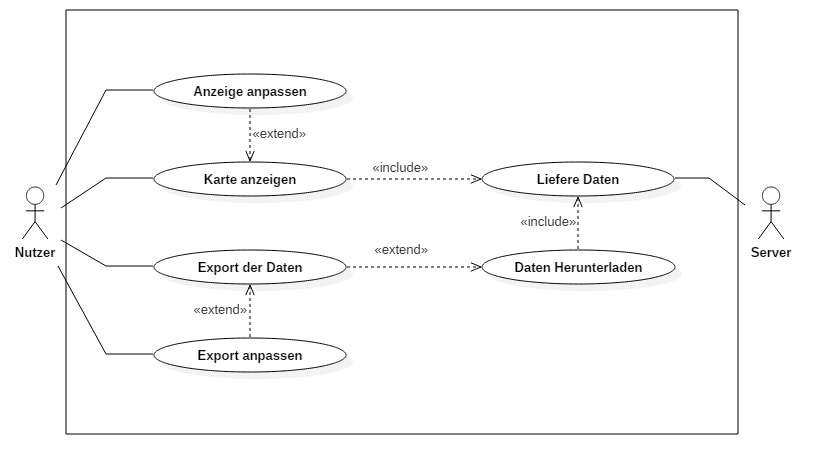
\includegraphics[width=1\linewidth]{diagrams/UseCaseDiagram1_Final.png}
       
       Dieser Anwendungsfall beschreibt die Bedienung des Webinterface. Dem Nutzer stehen folgende Aktionen zur Verfügung:
       \begin{itemize}
            \item Karte anzeigen
            \item Anzeige anpassen
            \item Daten exportieren
            \item Export anpassen
        \end{itemize}
        Nachdem der Nutzer auf das Webinterface zugreift, kann er sich die Karte anzeigen lassen. Diese visualisiert die Daten, welche 
        vom Server bereitgestellt werden. Die Anzeige der Karte, sowie des gesamten Interfaces lässt sich an die Wünsche des Nutzers 
        anpassen, beispielsweise durch die Einbeziehung von Graphen zur besseren Darstellung. Die Datenbestände lassen sich 
        herunterladen und in das gewünschte Format exportieren. Durch Beschränkung der Datenmengen auf bestimmte Zeitintervalle, 
        Datentypen und Wertebereiche kann der Export weiter angepasst werden.
        
    % Anwendungsfall Admin-GUI
    \subsection{Bedienung der Admin-GUI}
        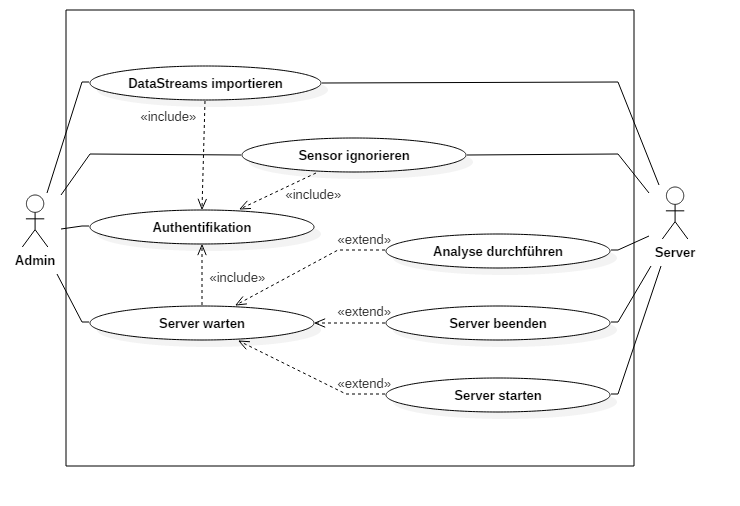
\includegraphics[width=1\linewidth]{diagrams/UseCaseDiagram2_Final.png}
        
        Dieser Anwendungsfall beschreibt die Bedienung der Admin-GUI. Dem Admin stehen folgende Aktionen zur Verfügung:
        \begin{itemize}
            \item Authentifikation
            \item Serverwartung
            \item DataStreams importieren
            \item Sensoren ignorieren
        \end{itemize}
        Um Zugriff auf die Funktionen des Admin-GUIs zu erhalten, muss sich der Admin zunächst authentifizieren. War dies erfolgreich, so 
        kann der Server gewartet werden. Der Admin kann ihn starten sowie beenden um Analysen durchzuführen und eventuelle 
        Fehler zu beheben. Weiterhin lassen sich DataStreams importieren, wodurch der Server diese verarbeiten und weiterverbreiten 
        kann. Dadurch können auch historische Datenbestände in den Datensatz aufgenommen werden. Auch hat der Admin die 
        Möglichkeit auszuwählen, welche Sensoren ignoriert werden, also wessen Daten nicht verbreitet und in den Datenbestand 
        aufgenommen werden sollen.
        
\section{Aktivitätsdiagramm}
    % Aktivitätsdiagramm
    \subsection{}
        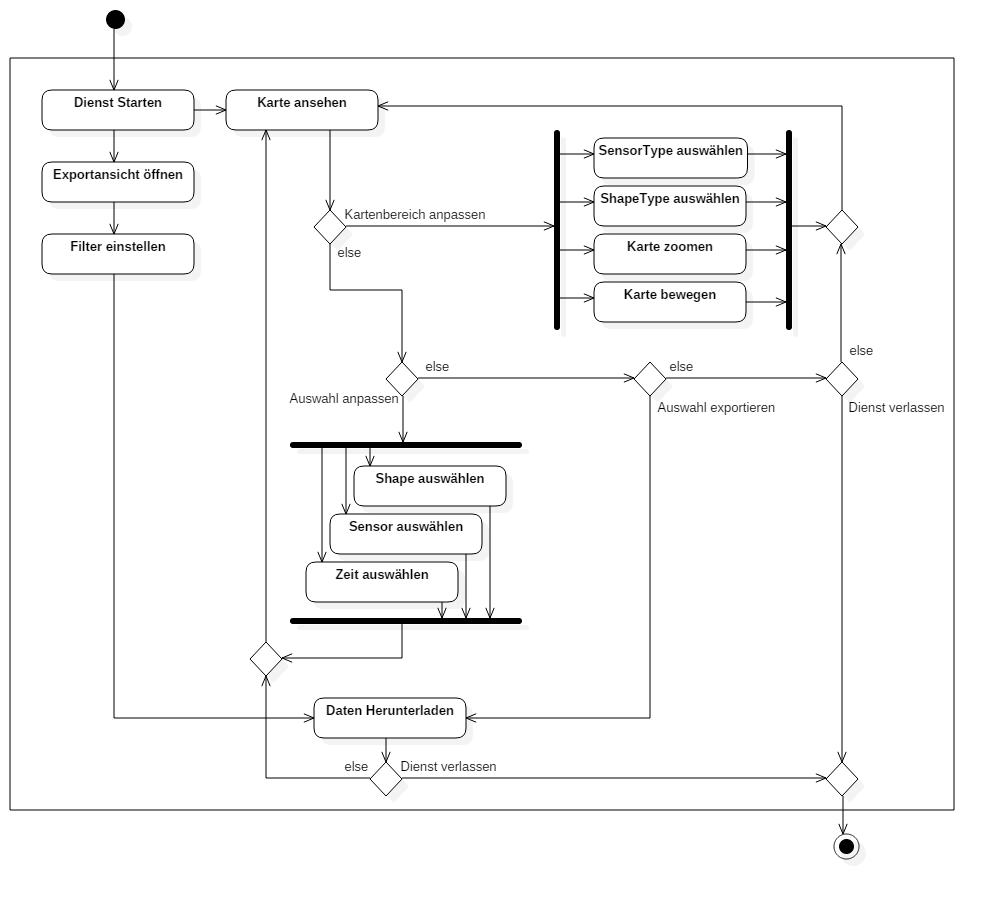
\includegraphics[width=1\linewidth]{diagrams/ActivityDiagram1_Final.png}

        